\documentclass[../5RO17_TP4.tex]{subfiles}

\begin{document}
\section{Visualisation de nuages de points}

\subsection{CloudCompare}
\noindent L'étape introductive de visualisation du nuage de points aide à comprendre la structure en trois dimensions d'un ensemble de points. Grâce à l'outil open source CloudCompare, on peut explorer la disposition spatiale des points, manipuler la structure pour observer les détails et analyser la géométrie.\\

\noindent Cette visualisation est essentielle pour saisir la complexité des formes et volumes dans un espace 3D, comme illustré avec les exemples de nuages de points du lapin ci-dessous:
\begin{figure}[H]
    \centering
    \begin{subfigure}[b]{0.325\textwidth}
        \centering
        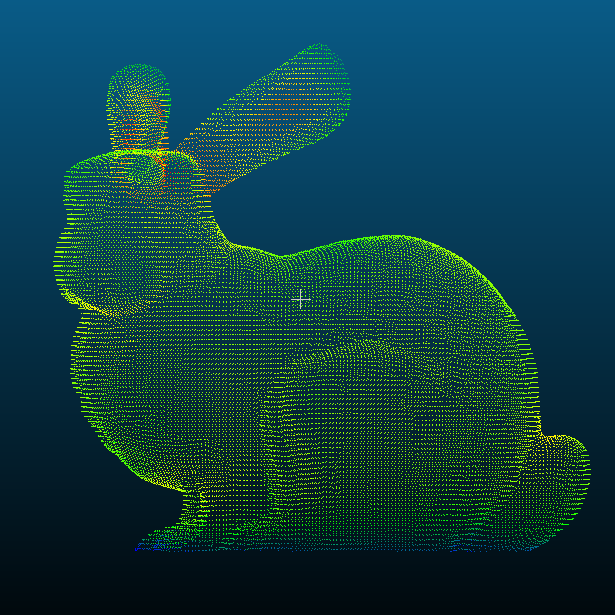
\includegraphics[width=\linewidth]{images/bunny_side.png}
        \caption{vue latérale}
        \label{}
    \end{subfigure}\hfill
    \begin{subfigure}[b]{0.325\textwidth}
        \centering
        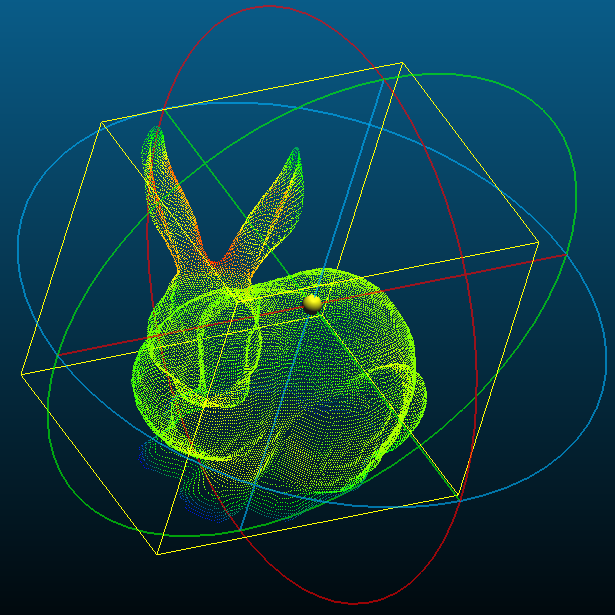
\includegraphics[width=\linewidth]{images/bunny_axis.png}
        \caption{degrés de liberté}
        \label{}
    \end{subfigure}\hfill
    \begin{subfigure}[b]{0.325\textwidth}
        \centering
        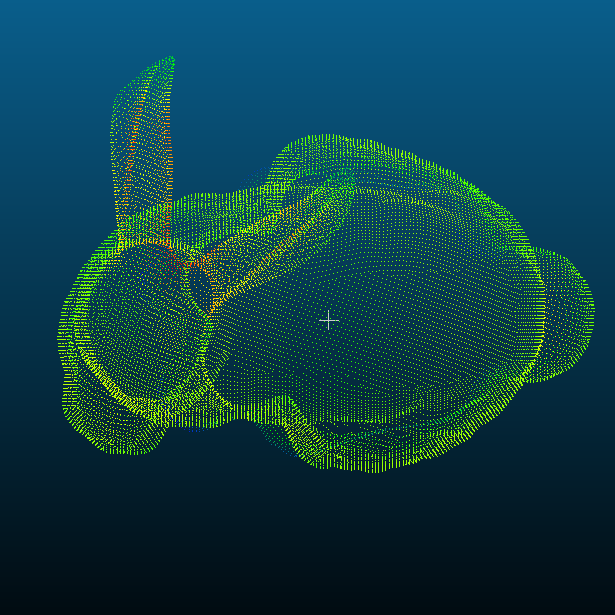
\includegraphics[width=\linewidth]{images/bunny_up.png}
        \caption{vue de dessus}
        \label{}
    \end{subfigure}
    \caption{Nuage de points \texttt{Bunny}}
    \label{}
\end{figure}
\noindent Pour des ensembles de données denses, comme le scan de Notre-Dame-des-Champs sur la Figure \ref{fig:sans_EDF}, la forte concentration de points et les couleurs par défaut peuvent masquer la perception de la profondeur. Pour remédier à cela, l'outil EDL, Eye Dome Lighting, de CloudCompare est utile.\\

\noindent Ce shader ajoute des contours et des ombres qui accentuent les variations de profondeur, offrant une visualisation plus nette et une perception de la tridimensionnalité renforcée sur la Figure \ref{fig:avec_EDF}.
\begin{figure}[H]
    \centering
    \begin{subfigure}[b]{0.475\textwidth}
        \centering
        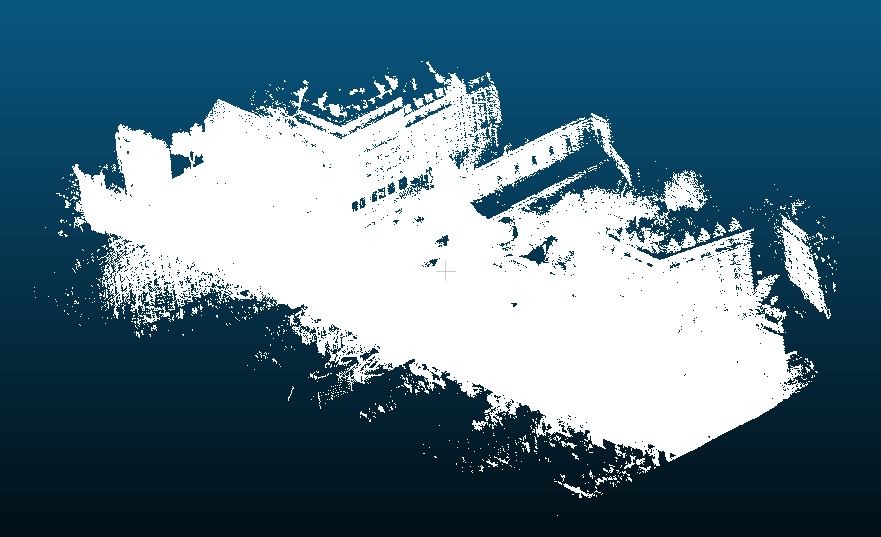
\includegraphics[width=\linewidth]{images/Notre.png}
        \caption{sans EDL}
        \label{fig:sans_EDF}
    \end{subfigure}\hfill
    \begin{subfigure}[b]{0.475\textwidth}
        \centering
        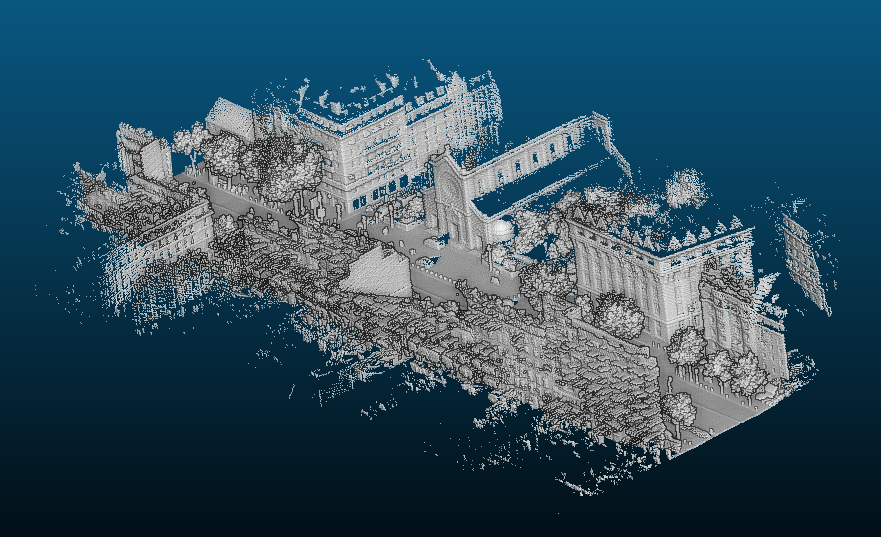
\includegraphics[width=\linewidth]{images/NotreEDL.png}
        \caption{avec EDL}
        \label{fig:avec_EDF}
    \end{subfigure}
    \caption{Nuage de points \texttt{Notre-Dame-des-Champs}}
    \label{fig:cloudcompare_ndc}
\end{figure}


\subsection{Python}
\noindent Il est également possible de visualiser et de manipuler ces nuages de points avec Python, comme nous le verrons dans les exercices suivants. Grâce aux bibliothèques \texttt{ply} pour la lecture des fichiers de nuages de points, \texttt{numpy} pour la manipulation de tableaux, et matplotlib pour l’affichage, nous pouvons créer, par exemple, les fonctions \texttt{read\_cloud} et \texttt{show\_cloud} présentées ci-dessous:

\begin{scriptsize}\mycode
	\begin{lstlisting}[language=Python, caption=\texttt{read\_cloud()}]
 def read_cloud(path: str) -> np.ndarray[float]:
    data_ply = read_ply(path)

    return np.vstack((data_ply['x'], data_ply['y'], data_ply['z']))
	\end{lstlisting}
\end{scriptsize}

\begin{scriptsize}\mycode
	\begin{lstlisting}[language=Python, caption=\texttt{show\_cloud()}]
def show_cloud(
        points: np.ndarray[float], title: str = 'Cloud of Points', save: bool = False
    ) -> None:
    fig = plt.figure()
    ax = fig.add_subplot(111, projection='3d')

    ax.scatter(
        points[0], points[1], points[2], s=0.1, c='b', marker='o', label=f'{points.shape[1]} points'
    )

    ax.set_xlabel('x', fontsize=12)
    ax.set_ylabel('y', fontsize=12)
    ax.set_zlabel('z', fontsize=12)

    ax.view_init(elev=30, azim=-45)

    ax.set_title(f'{title}', fontsize=14)
    ax.legend(loc='upper left')

    plt.tight_layout()

    if save:
        file_path = os.path.abspath(os.path.join(os.getcwd(), f'../outputs/{title}.png'))
        plt.savefig(file_path, dpi=300)

    plt.show()
	\end{lstlisting}
\end{scriptsize}
\noindent Ces fonctions permettent une représentation tridimensionnelle des points sur la Figure \ref{fig:python_plots} et offrent des fonctionnalités de translation, de rotation et de zoom similaires à celles de CloudCompare comme indiqué ci-dessous:
\begin{figure}[H]
    \centering
    \begin{subfigure}[b]{0.475\textwidth}
        \centering
        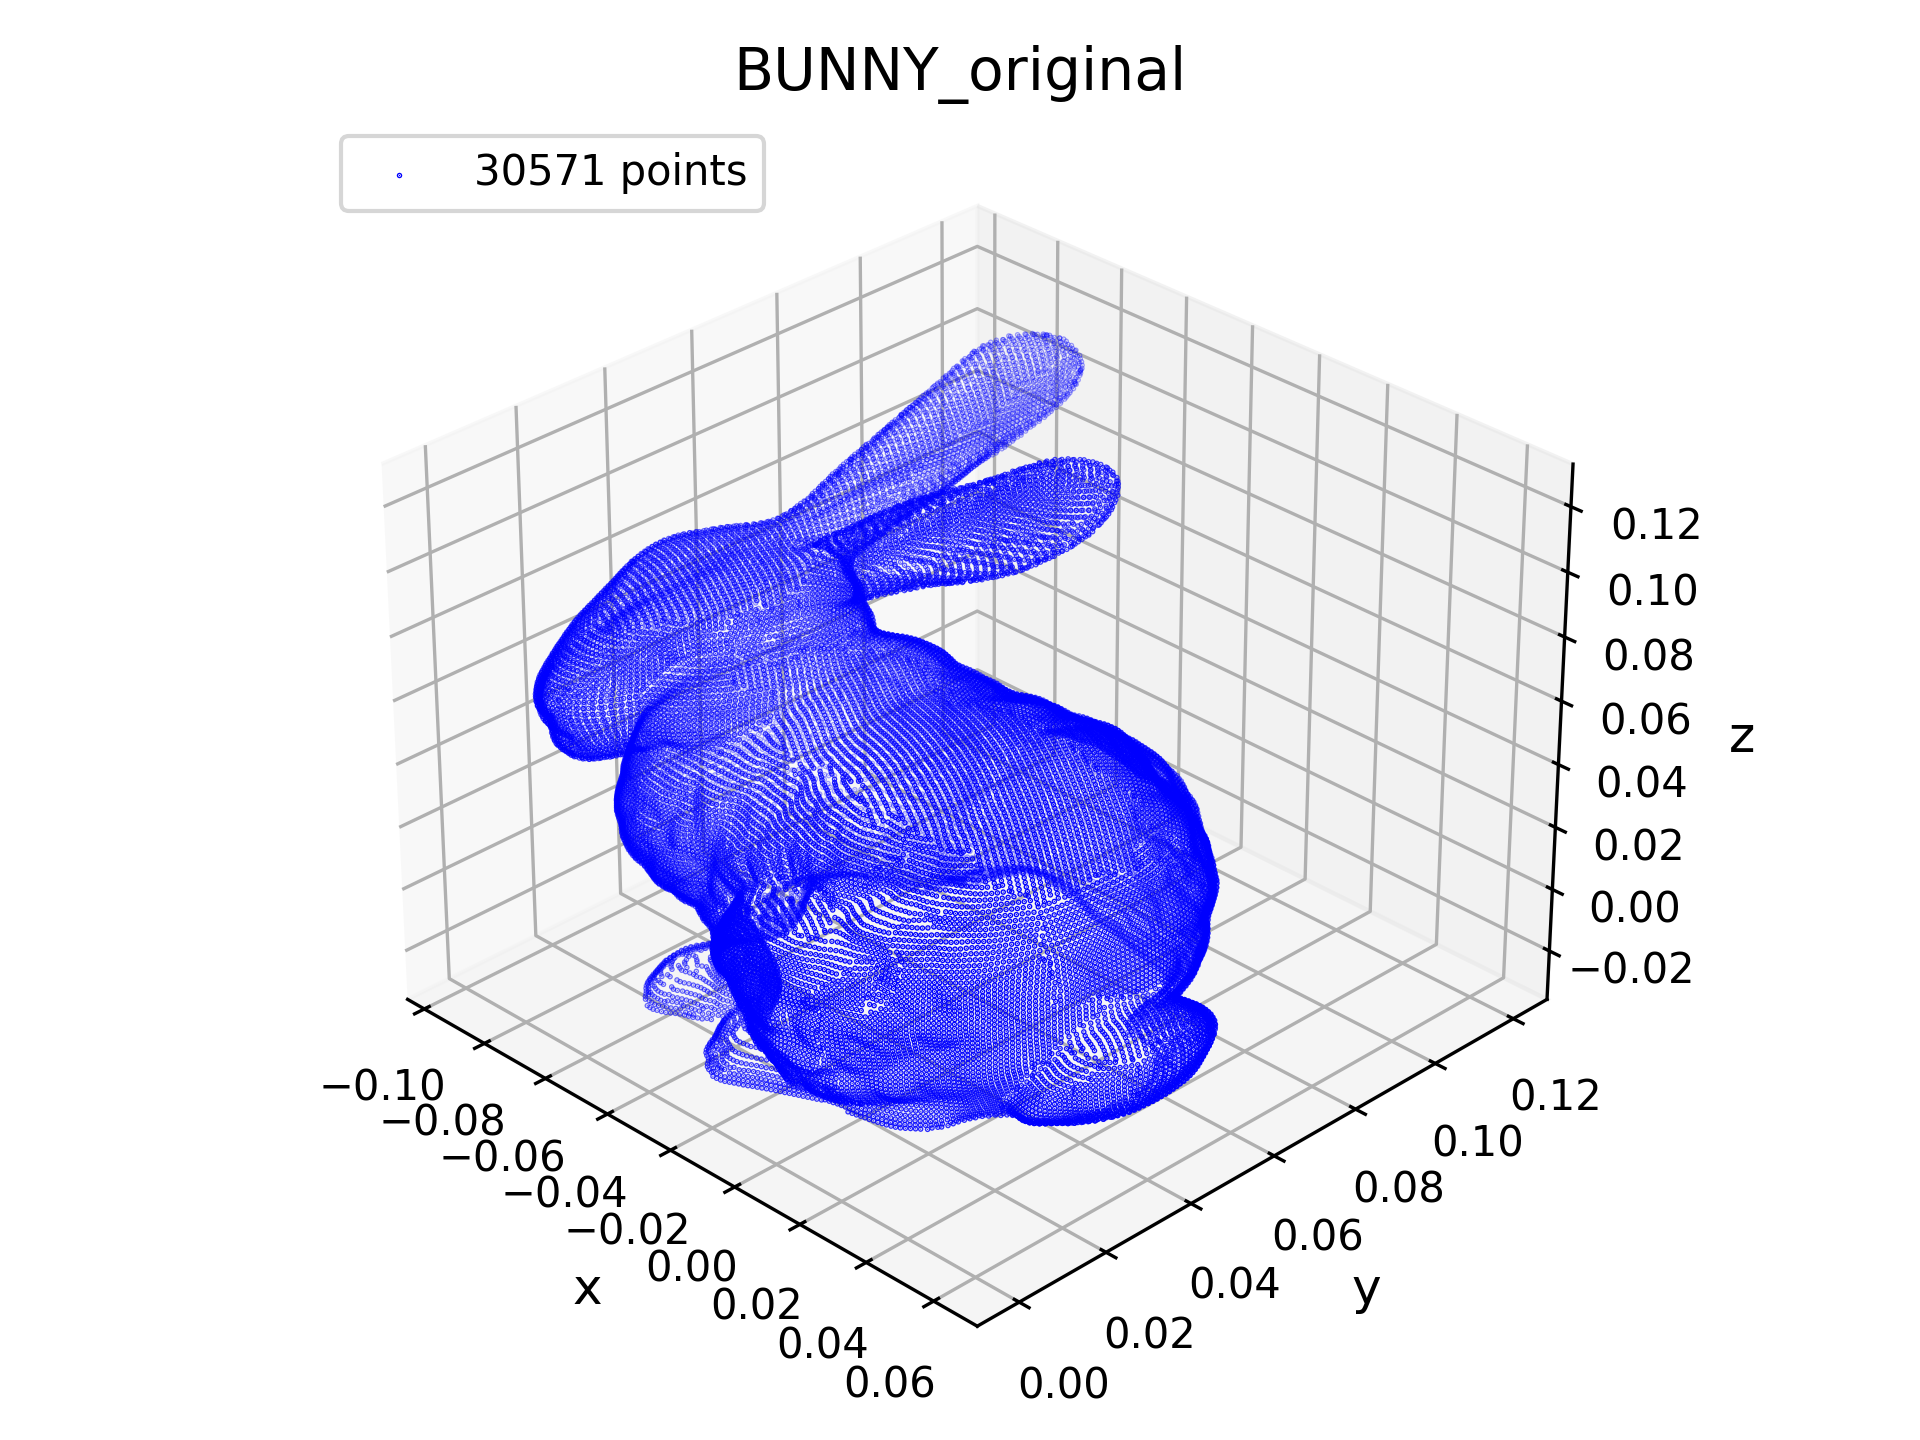
\includegraphics[width=\linewidth]{images/BUNNY_original.png}
        \caption{Bunny}
        \label{fig:python_bunny}
    \end{subfigure}\hfill
    \begin{subfigure}[b]{0.475\textwidth}
        \centering
        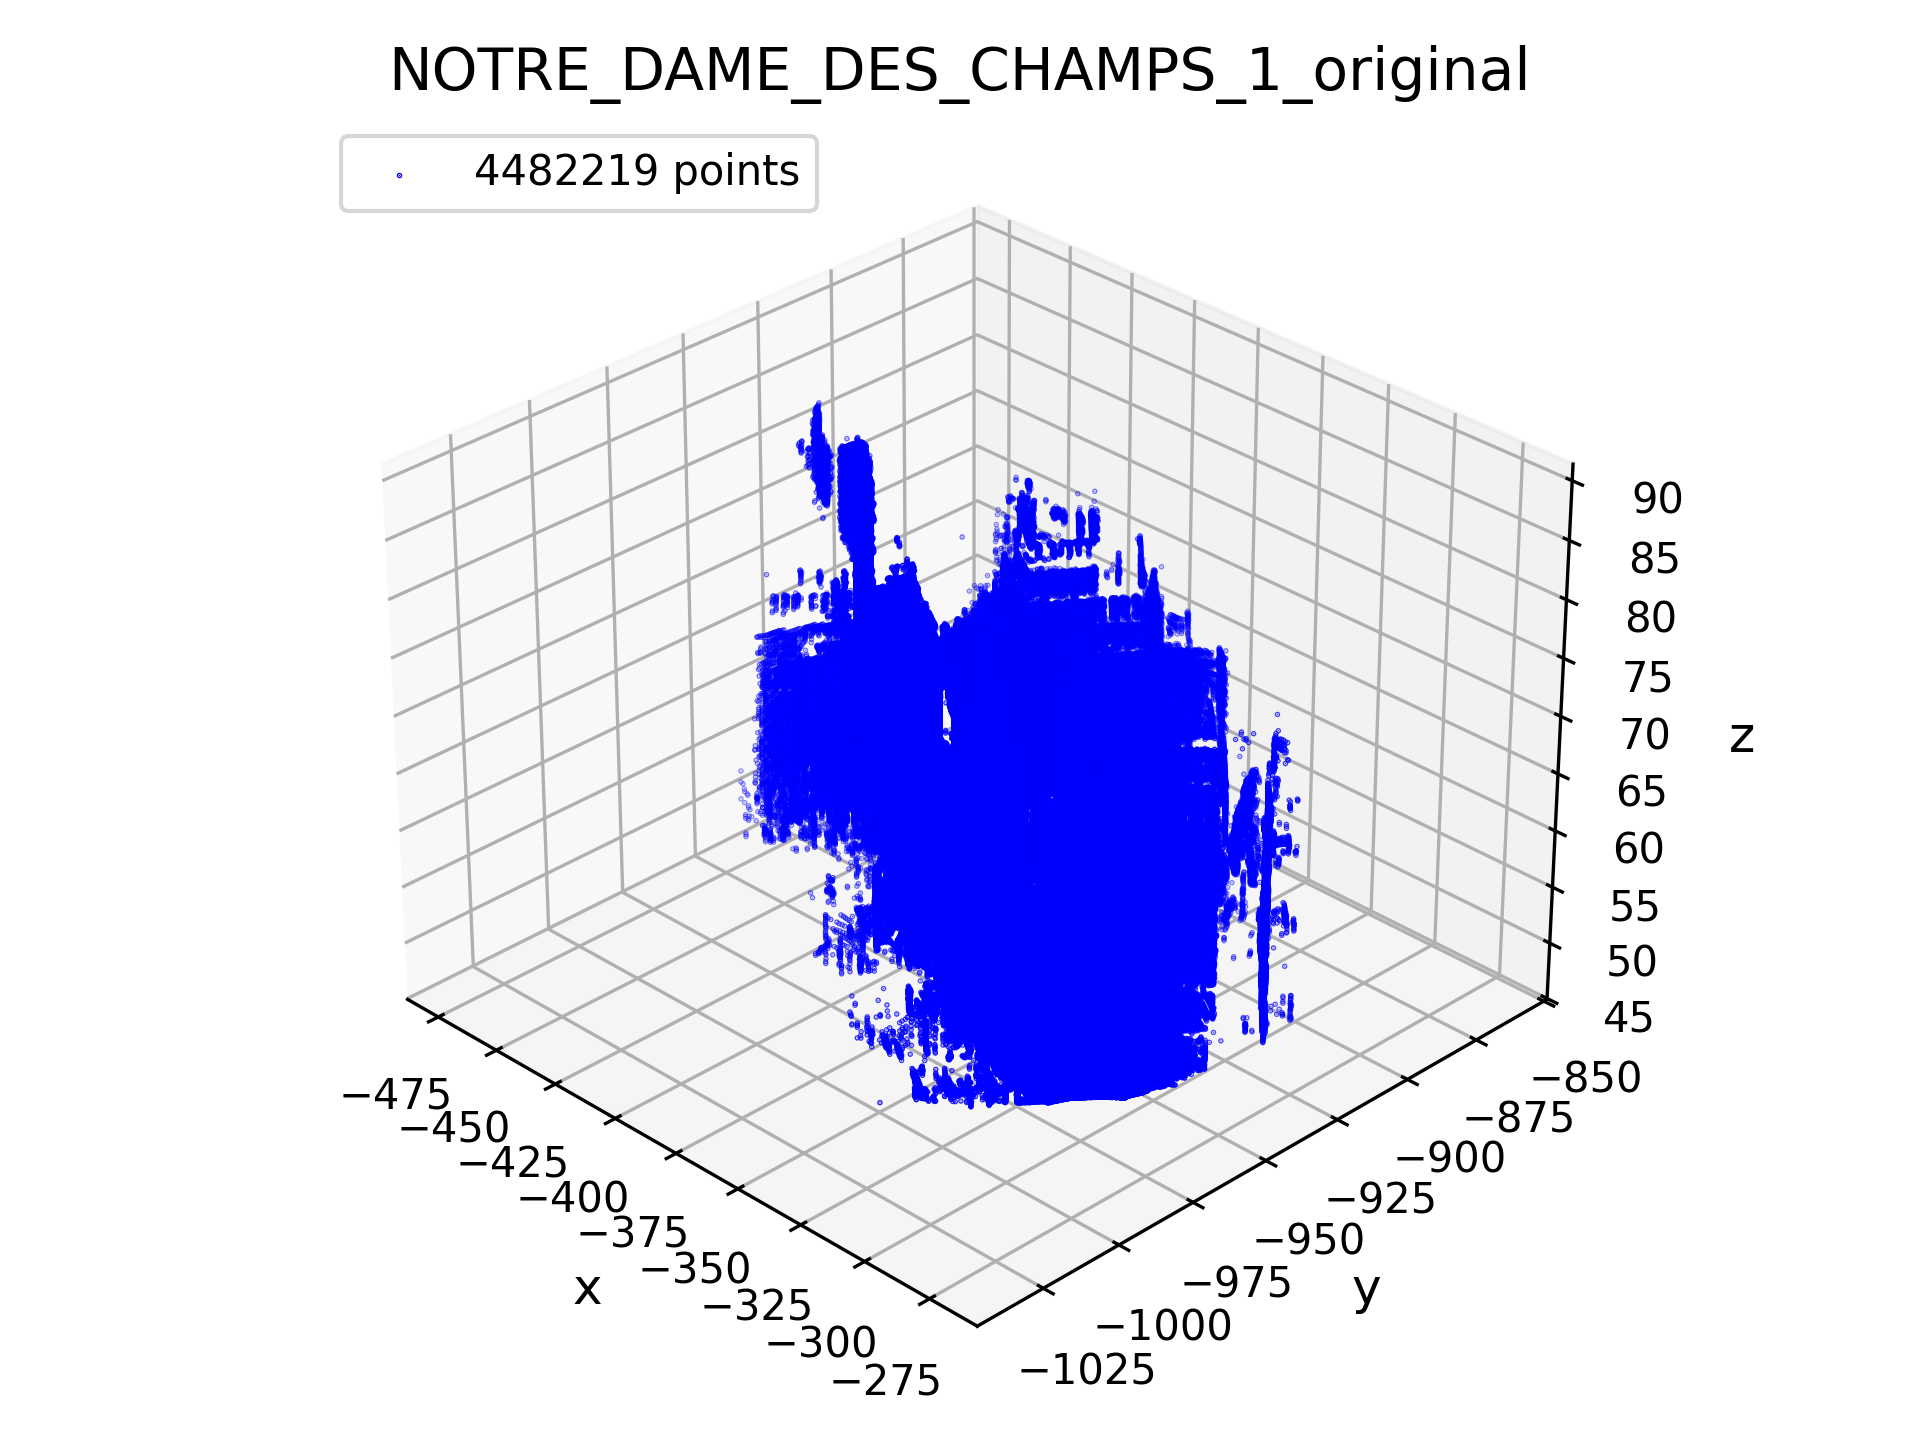
\includegraphics[width=\linewidth]{images/NOTRE_DAME_DES_CHAMPS_1_original.png}
        \caption{Notre-Dame-des-Champs}
        \label{fig:python_ndc}
    \end{subfigure}
    \caption{Visualization nuage des points avec Python}
    \label{fig:python_plots}
\end{figure}
\noindent Il est notable qu'il est possible de compreendre le résultat visuel pour un petit nuage des points, mais pour un nuage de grande taille, l'interprétation devient moins claire. De plus, le temps de calcul requis pour ouvrir e manipuler un grand ensemble de données est considérablement plus long avec cette méthode.
\end{document}
